% This LaTeX was auto-generated from MATLAB code.
% To make changes, update the MATLAB code and export to LaTeX again.


\documentclass{scrreprt}

\usepackage{geometry}
\usepackage[utf8]{inputenc}
\usepackage{blindtext}
\usepackage[T1]{fontenc}
\usepackage{lipsum}
\usepackage{hyperref}
\usepackage{enumitem}
\usepackage{graphicx}
\usepackage{float}
\usepackage{hyperref}

\hypersetup{
    colorlinks=true,
    linkcolor=blue,
    filecolor=magenta,      
    urlcolor=cyan,
}

\urlstyle{same}

\newlength\mylen
\setlength\mylen{0.5in}
\geometry{letterpaper, portrait, lmargin=1.5in, tmargin=1in}

\renewcommand*{\chapterformat}{%
  \llap{\protect\makebox[\mylen][l]{\chapappifchapterprefix{\nobreakspace}\thechapter\autodot\hfill}}%
}






\begin{document}

\chapter{Introduction}


\section{Purpose}
The purpose of this document is to describe the operating steps, description theory, and fault isolation procedures of the microdroplet impact analysis software. 


\section{Document Conventions}
\lipsum[4]

\section{Intended Audience}
MATLAB Microdroplet Impact Analysis Application is designed for students, professors, professionals, and anyone interested in analyzing microdroplet impacts. This application was initially designed for Interfacial Fluid Dynamics Lab at Washington State University Vancouver. However, this is an open source program and can be used by anyone. 

\section{Product Scope}
This applet is to be used for automated processing of microfluid droplet videos. This applet takes an input of .avi video files and provides a table of parameters for instantaneous primary droplet velocity, primary droplet spread radius, satellite droplet velocity, number of satellite droplets per frame, jet velocity, jet diameter, jet tip position, primary droplet contact angle, maximum primary droplet spread radius, and maximum primary droplet velocity. This data is intended for use in aiding research in microfluid behavior. This applet is not intended to replace logical reasoning, so data taken from this applet should be checked before use in academic research in case errors have occurred in processing.























\chapter{Overall Description}


\section{Product Perspective}
This applet reduces the need for extensive image processing training and coding for researchers, as it provides much of the basic parameters that are necessary for microfluid droplet analysis. However, this applet is a living code that needs continuous updates to be compatible with a wide range of droplet videos. At its current iteration, this applet can be used on droplets with high contrast against their environment that move vertically from the perspective of the camera.

\section{Product Functions}
The applet can be used to output:
\begin{itemize}
\item Basic microdroplet parameters, such as:
\begin{itemize}
\item primary and satellite droplet velocity
\item primary droplet spread radius
\item primary droplet contact angle
\item jet speed
\item jet diameter
\item jet tip position
\item number of satellite droplets
\end{itemize}

\item Individual processed frames with either droplet outlines or contact angle lines.

\end{itemize}

\section{User Classes and Characteristics}
The user classes for this applet include undergraduate, graduate, and postgraduate researchers as well as university instructors and researchers. Undergraduate researchers are likely to be using laptops or other computers with limited memory resources. These users will also be performing introductory levels of analysis of microfluid droplet behavior. Graduate, postgraduate, and university researchers are likely to have access to high performing computing, such as that provided by computing clusters. These users are likely to be performing higher level analysis of microfluid droplet behavior and are more likely to be able to spot processing errors if they arise. For all user classes, this applet provides many of the key parameters necessary for conducting microfluid droplet analysis without the need to learn image processing algorithms or extensive MATLAB coding tools.

\section{Operating Environment}
This applet was created in MATLAB, which has been tested on Mac, Windows, and Ubuntu operating systems. This applet was created and tested using Windows.

\section{Design and Implementation Constraints}
This applet is constrained to use on microfluid droplet videos in the .avi format. Future iterations may be implemented for use with a wider range of video formats. The applet is also unable to process droplets that are clear or provide little contrast to the background. Input videos must be converted to grayscale prior to use in the applet. The user is expected to provide high quality input videos for optimal processing.

\section{User Documentation}
Any user of this applet is the target audience of this user documentation. For users that may be altering the code of the GUI or image processing functions, additional documentation found on the MathWorks website is suggested as a supplemental resource.

\section{Assumptions and Dependencies}
It is assumed that all users of this applet have at least a basic understanding of microfluid analysis and an ability to understand MATLAB error messages. 

\chapter{GUI User Guide}
In this chapter, a step-by-step guide for the use of the GUI is provided, with images.

\section{Installation}

\begin{enumerate}[label = Step \arabic*.]

\item Double left-click on GUI\_Design.mlappinstall. \\
\item Left-click on "Install" on pop-up window.
\begin{figure}[H]
\centering
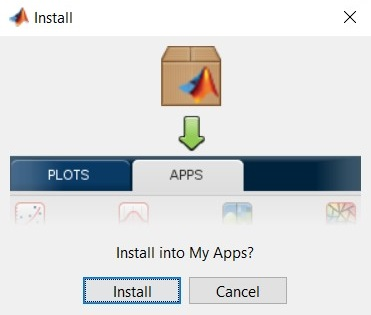
\includegraphics[width=0.5\textwidth]{InstallIntoMyApps.jpg}
\label{fig:installpopup}
\end{figure}
\end{enumerate}

\section{Opening the Applet}

\begin{enumerate}[label = Step \arabic*.]

\item Open MATLAB. \\
\item Left-click on the "APPS" tab in the top left corner of the MATLAB environment
\begin{figure}[H]
\centering
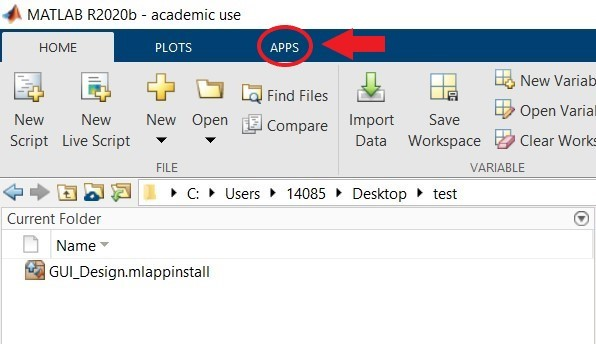
\includegraphics[width=0.5\textwidth]{FindingApps.jpg}
\label{fig:appstablocation}
\end{figure} 

\item Left-click on the dropdown menu in the APPS bar.
\begin{figure}[H]
\centering
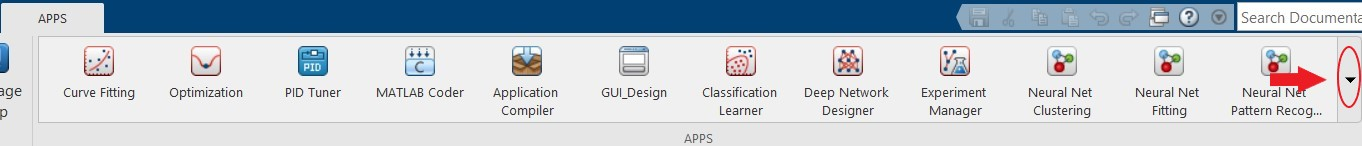
\includegraphics[width=\textwidth]{APPSDropDown.jpg}
\label{fig:appsdropdown}
\end{figure}

\item From the dropdown menu, left-click GUI\_Design from the "MY APPS" section.
\begin{figure}[H]
\centering
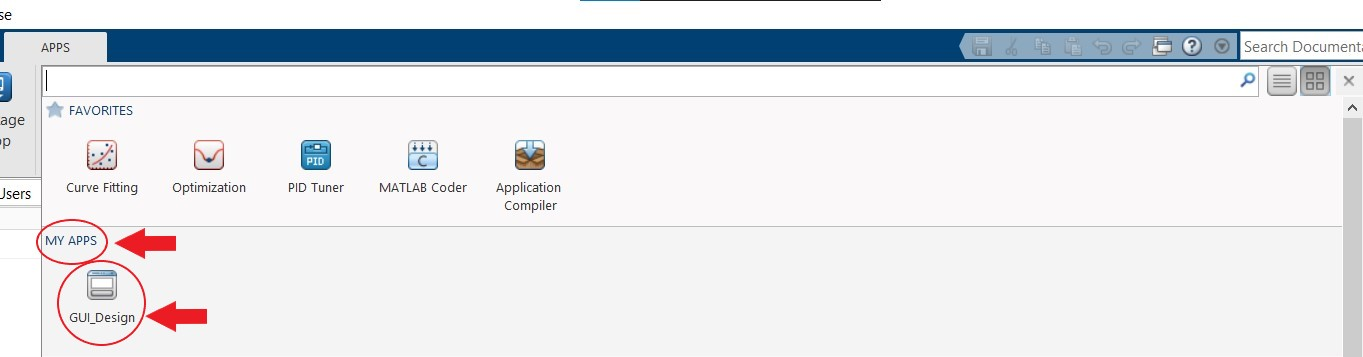
\includegraphics[width=0.5\textwidth]{MyAppsSection.jpg}
\label{fig:myappssection}
\end{figure}

\end{enumerate}

\section{Using the Applet}

\subsection{Uploading a Video}

\begin{enumerate}[label = Step \arabic*.]

\item Left-click on the "Upload Video" button. 
\begin{figure}[H]
\centering
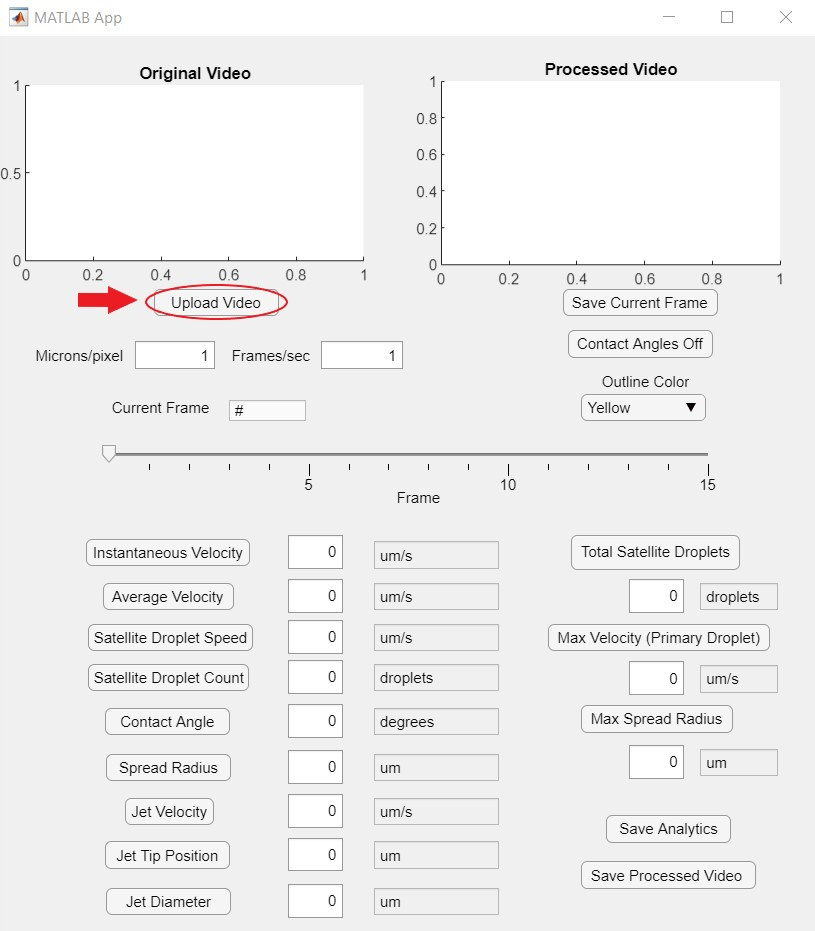
\includegraphics[width=0.5\textwidth]{appletbeforeupload.jpg}
\label{fig:uploadvideobutton}
\end{figure}

\item Select the video you would like to upload from the File Explorer window. Select "Open" to open that video file in the applet. The applet will open a secondary window for floor selection. You can either use the interactive floor finding or input the floor height in pixels and the floor angle. \\

\end{enumerate}

\subsubsection{Interactive Floor Finding}
\begin{enumerate}[label = Step \arabic*.]

\item Left-click the "Start Interactive Floor Find" button.
\begin{figure}[H]
\centering
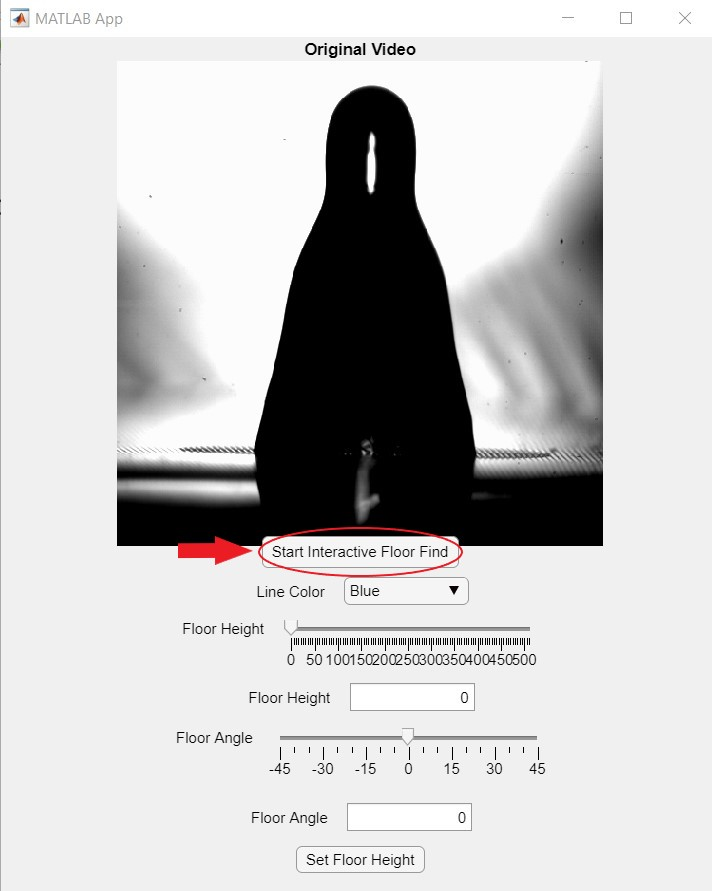
\includegraphics[width=0.5\textwidth]{SecondaryAppletFloorFindButton.jpg}
\label{fig:interactivefloorfindbutton}
\end{figure}

\item An instructional message will appear, informing the user that they can now draw a line at the floor on the video frame. Press the "OK" button to proceed with the interactive floor finding.
\begin{figure}[H]
\centering
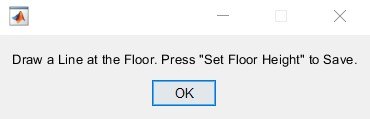
\includegraphics[width=0.5\textwidth]{DrawALineMsg.jpg}
\label{fig:drawalinemsg}
\end{figure}

\item Left-click and drag on the image to draw a line for the floor. To move this line, left-click and drag either blue dot at the ends of the line. Use the "Zoom-In" feature in the upper right-hand corner of the image to get a better look at where the floor line is located on the image. Continue manipulating the line by moving the blue dots until the interactive floor line matches the line of the floor in the original image. Press "Set Floor Height" Button once the interactive line is aligned.

\begin{figure}[H]
\centering
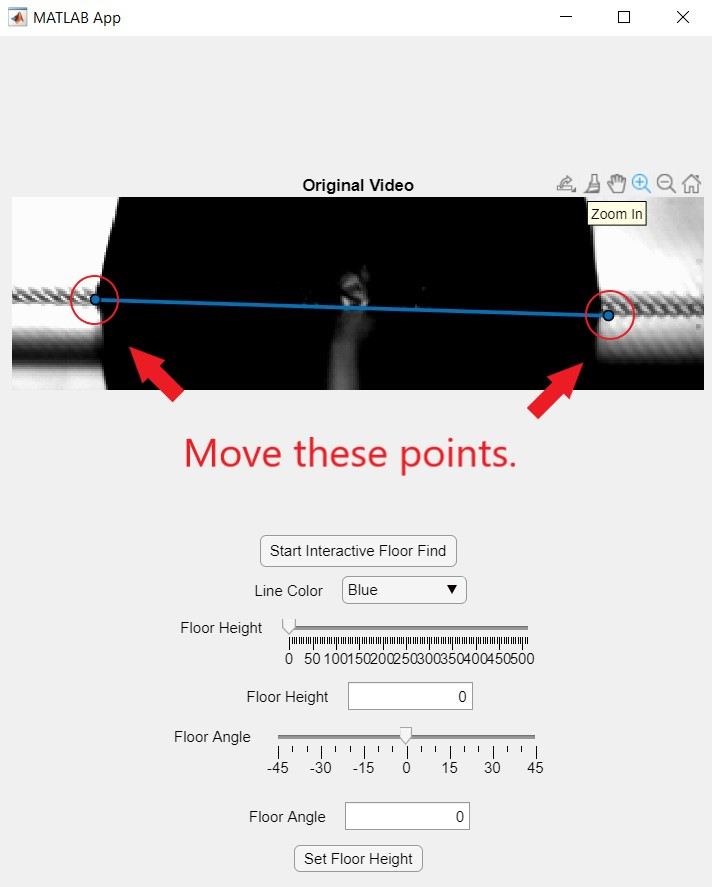
\includegraphics[width=0.5\textwidth]{InteractiveFloorLine.jpg}
\label{fig:interactiveline}
\end{figure}

\subsubsection{Manual Floor Height and Angle Entry}
During the manual floor height and angle entry process, if the line is difficult to see, the user can select a different line option from the "Line Color" dropdown menu. This feature is ONLY available for the line printed by manual floor height and angle entry.


\item Move the slider next to "Floor Height" or manually enter floor height value into the textbox below to set a floor height. Note: "Floor Height" is measured in pixels, counting the number of pixels from the top of the image to the centermost pixel of the floor line.
\begin{figure}[H]
\centering
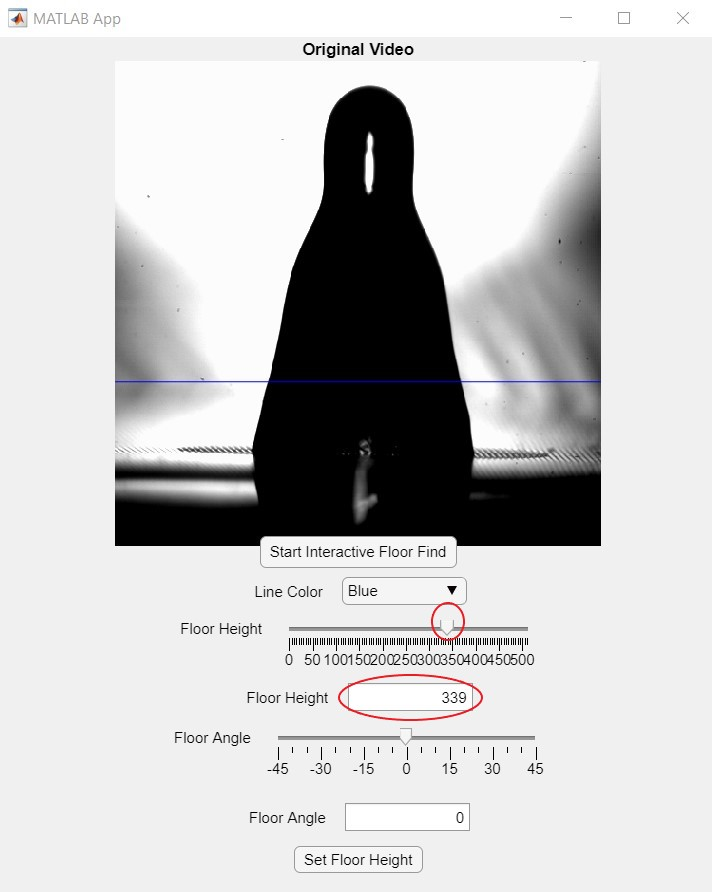
\includegraphics[width=0.5\textwidth]{ManualFloorHeight.jpg}
\label{fig:manualfloorheightslct}
\end{figure}

\item Move the slider next to "Floor Angle" or manually enter floor angle value into the textbox below to set a floor angle. 
\begin{figure}[H]
\centering
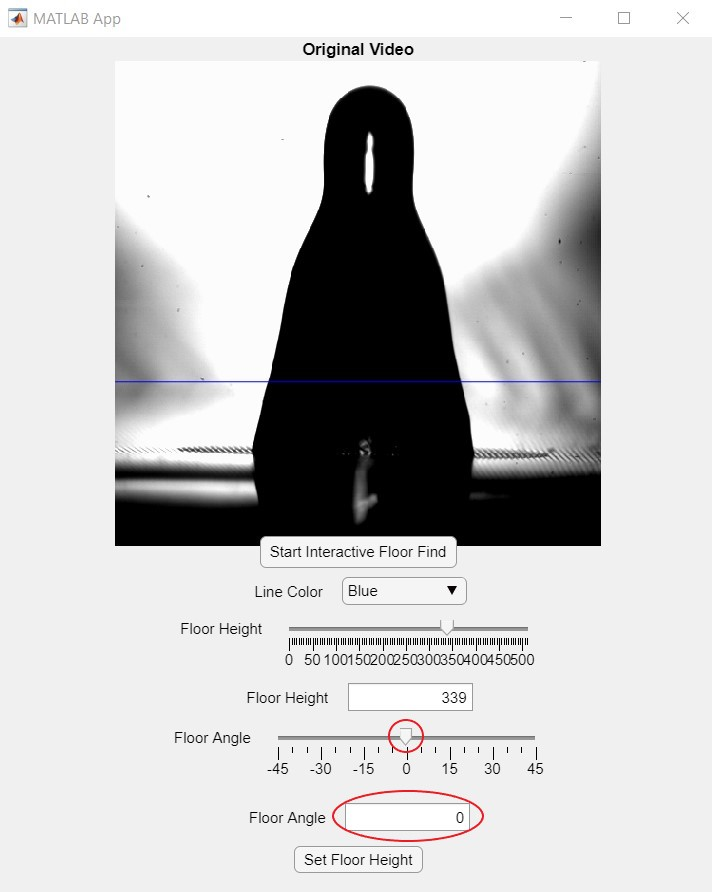
\includegraphics[width=0.5\textwidth]{ManualFloorAngle.jpg}
\label{fig:manualfloorangleslct}
\end{figure}

\item Once both floor height and floor angle are at the correct values, left-click the "Set Floor Height" button to input the floor values.

\item Once the floor height and angle has been set, the applet will process the entire video, then display the processed video. Please note, this process takes a lot of computation and will take time, especially on computers with limited processing power. 
\begin{figure}[H]
\centering
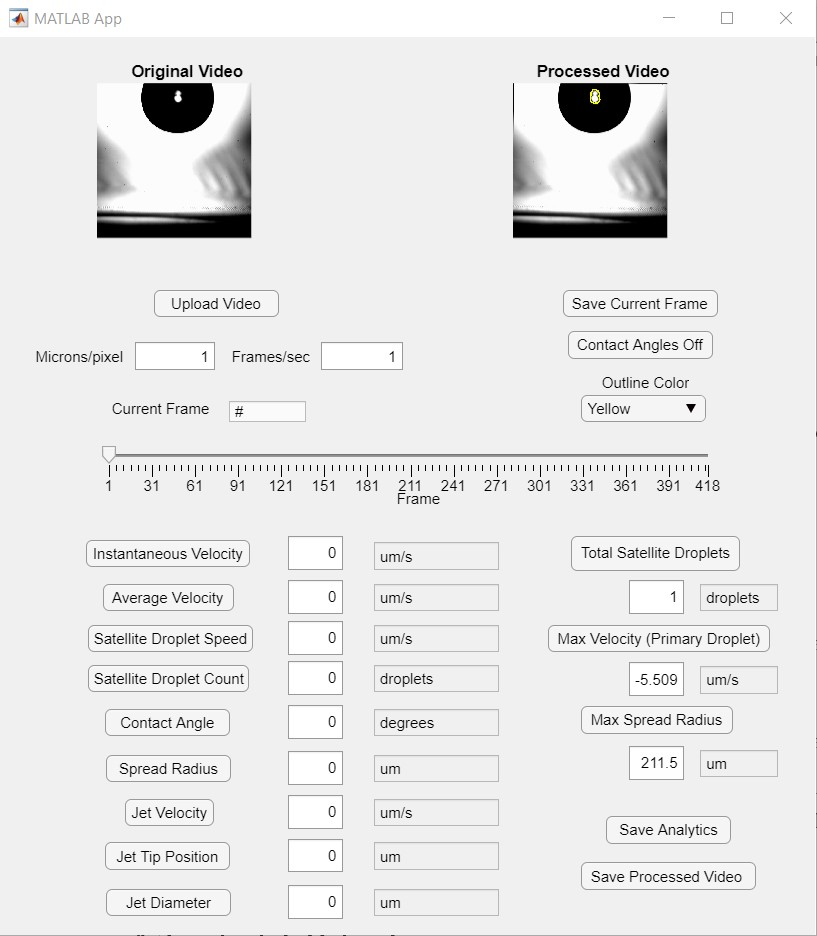
\includegraphics[width=0.5\textwidth]{FirstProcessedVideoImage.jpg}
\label{fig:rightafterfloorfind}
\end{figure}
\end{enumerate}

\subsection{Applet Features}












\chapter{System Functions}
In this chapter each of the image processing and droplet analysis functions are described. A paragraph of the system theory is given and describes the overall operation of the function and the variables in it. A fault isolation section is also provided which gives solutions and fixes to possible issues that may arise. 

\section{borders}
\label{sec:borders}
\subsection{Theory and Description}
The borders function is the second video processing function applied to the source video. 

\subsection{Fault Isolation}
\lipsum[4]



\section{fallVelocity}
\label{sec:fallVelocity}
See also: \hyperref[sec:video2frame]{video2frame}, \hyperref[sec:floorremove]{floorremove}, \hyperref[sec:borders]{borders}
\subsection{Theory and Description}
The function fallVelocity finds and tracks the centroids and velocities of all objects in an input four dimensional borders matrix of data type uint8. This function finds the speed and frame of impact of the main droplet, records the centroids and velocities of all tracked objects per frame, and tracks the total number of satillite objects found in the video.The function can be called as follows:
\begin{verbatim}
[dropletVelocity, impactData, numberOfSatillites] = 
fallVelocity(videoFloorRemoved, floorHeight)
\end{verbatim}  
 Where numberOfSatillites is an integer number of satillite droplets in the video, impactData is a two element array where the first element is the downwards velocity of the first droplet at impact as a double and the second element is the frame at which the droplet made impact, and dropletVelocity is a three dimensional array of the size [4,numberOfSatillites+1,Frames]. dropletVelocity is formatted as follows:
\begin{verbatim}
[Centroid1_X, Centroid2_X, Centroid3_X, Centroid4_X;...
 Centroid1_Y, Centroid2_Y, Centroid3_Y, Centroid4_y;...
 Velocity1_X, Velocity2_X, Velocity3_X, Velocity4_X;....
 Velocity1_Y, Velocity2_Y, Velocity3_Y, Velocity4_Y...]
\end{verbatim} 
videoFloorRemoved is the 4 dimensional matrix output from the floorremove function. floorHeight is the value tracking the height of the floor; it is used to find the frame of impact.

\subsection{Fault Isolation}
This functions currently does not have fault isolation. This function needs to be able to reliably identify and track droplets even when they pass off screen. This has not been implemented, and may cause errors. In addition, the floor impact data relies heavily on the floorremove function. If there are errors, check floorremove and floor GUI.

\section{contactAngles}
\label{sec:contactAngles}
See also: \hyperref[sec:video2frame]{video2frame}, \hyperref[sec:floorremove]{floorremove}, \hyperref[sec:borders]{borders}, \hyperref[sec:drawContactAngles]{drawContactAngles}
\subsection{Theory and Description}
The function contactAngles finds the angles of the contact the droplet has with the floor and the locations of contact. This function can be callled as follows:
 \begin{verbatim}
[contactAngle, contactPoints] =
contactAngles(imageFloorRemoved, floorHeight, numberOfPoints,polyOrder)
\end{verbatim}  
The inputs are the following: imageFloorRemoved, the 4 dimensional matrix from the floorremoved function; foorHeight, the floor pixel height used in the floorremoved function; numberOfPoints, the number of sample points along the edge of the droplet to calculate the contact angles. Default: 10; polyOrder, the polynomial order used to calculate the contact angles. Default: 2. numberOfPoints must always be greater than polyOrder. 
The outputs are as follows: contactAngle is a 2 dimensional matrix of the size [2,Frames]. The first value of contactAngles is the right contact angle, while the second value is the left contact angle. contactPoints is a 3 dimensional of the size [2,2,frames]. contactPoints is formatted as follows:
\begin{verbatim}
contact[1,:,:] is the right contact point
contact[2,:,:] is the left contact point
contact[:,1,:] is the x value
contact[:,2,:] is the y value
\end{verbatim}
The contactAngles function works by collecting a series of points on either side of the droplet once it has contacted the floor. Those points are then used to create a polyfit estimation of the curve of the droplet. Once the derivative of the polyfit is found the slope at each contact point, found using the floorHeight imput, is calculated. The slopes are converted into degrees and saved.


\subsection{Fault Isolation}
contactAngles as two optional inputs. If numberOfPoints and polyOrder are not entered, that is:
 \begin{verbatim}
[contactAngle, contactPoints] =contactAngles(imageFloorRemoved, floorHeight)
 \end{verbatim}
then default values for those inputs are used. There is no error checking to ensure that the found contact angles make sense. Instead, those additional options were created to allow for more refined configurations. contactAngles relies heavily on floorremove. If the user input floorremove settings are inaccurate, this function will be prone to create errors.

\section{convertSource}
\label{sec:convertSource}
See also: \hyperref[sec:video2frame]{video2frame}, \hyperref[sec:floorremove]{floorremove}, \hyperref[sec:maskOverlay]{maskOverlay}
\subsection{Theory and Description}
The function convertSource converts an input video frame matrix, referred to as videoSource, to an RGB video frame matrix of data type of unint8. This function also rotates videoSource to match the rotation of of the analyzed frames. The function can be called as follows:
\begin{verbatim}
convertedVideoSource = convertSource(videoSource, floorAngle)
\end{verbatim}  
Where convertedVideoSource is a four dimensional matrix of data type uint8 and the form [Height, Width, 3, Frame]. convertedVideoSource is the same size as videoSource, but has a video mode of 3. floorAngle is given in degrees.
\subsection{Fault Isolation}
This function is compatible with RGB24 and greyscale videoSource matrices for future compatibility. If videoSource is off the wrong format, not a 4 dimensional matrix or videoMode is not either 1 or 3, this function will halt and report the following error: \\
\textbf{'Unexpected Source Matrix format. Please provide a grayscale image, an RGB image, or a binary image.'} \\
If you receive this error, videoSource may have been changed after video2frame, or video2frame encountered an uncaught error importing the video. 

\section{drawContactAngles}
\label{sec:drawContactAngles}
See also: \hyperref[sec:maskOverlay]{maskOverlay}, \hyperref[sec:outlineMask]{outlineMask}, \hyperref[sec:contactAngles]{contactAngles},
\subsection{Theory and Description}
The function drawContactAngles creates a post-processing video frame matrix mask showing the contact angles with a predefined line length. The returned video mask is boolean black-and-white 4D video matrix of the height, width, and length defined by the videoSize input. The function can be called as follows:
\begin{verbatim}
maskAngle = drawContactAngles(videoSize, contactAngle, contactPoints, lineLength)
\end{verbatim}  
Where videoSize is a 4 element integer array of the form [Height, Width,videoMode,Frames], contactAngle is the contact angle matrix from the contactAngles function, contactPoints is the contact position matrix from the contactAngles function, and lineLength is an interger line length.\\ \\
drawContactAngles creates this contact angle video mask by first creating a 4 dimensional boolean matrix of the size [videoHeight, videoWidth, 1, videoLength] set to false. Each contact angle in each frame is defined by the variables lineX and lineY, where lineX is an array of linearly spaced integer x-axis values between\\
$(contactPointInX\pm LineLength*Cos[contactAngle])$\\
lineY is a similiar array in the vertical direction with the same number of elements. Together lineX and lineY make up linearly spaced integer coordinate pairs. If either value in each coordinate pair is outside the height or width range of the video, that pair is removed from the set {[lineX,lineY]}. The {[lineX,lineY]} coordinate pairs are then used to set the corresponding pixels in each frame to true. This process is repeated for each contact point in each frame of the video.
\subsection{Fault Isolation}
By removing any points that are outside of the given range, the video mask matrix will always match the videoSize dimensions provided. This function can handle non-integer lineLength values, but it will be rounded down to the nearest odd number. This function skips drawing contact angles for frames where either the contact point or the contact angle is undefined, meaning this function works when there are no contact angles to draw. There is no error checking for the videoSize inputs.
 



\section{calculateVelocity}
\label{sec:calculateVelocity}
\subsection{Theory and Description}
\lipsum[4]

\subsection{Fault Isolation}
\lipsum[4]




\section{floorremove}
\label{sec:floorremove}
\subsection{Theory and Description}
\lipsum[4]

\subsection{Fault Isolation}
\lipsum[4]




\section{frame2file}
\label{sec:frame2file}
See also: \hyperref[sec:floorremove]{floorremove}, \hyperref[sec:video2frame]{video2frame}, \hyperref[sec:convertSource]{convertSource}, \hyperref[sec:maskOverlay]{maskOverlay}
\subsection{Theory and Description}
frame2file takes a frame from a video frame matrix and saves it as an image file at a chosen location. This function is compatible with RGB24 and greyscale video frame matrices. The file may be saved as .bmp, .gif, .hdf, .jpg, .jpeg, .jp2, .jpx, .pbm, .pcx, .png, .pnm, .ppm, .ras, .tif, .tiff, or .xwd. This function can be called as follows:
\begin{verbatim}
frame2file(videoToBeSaved, your_file_name.ext, 'C:\your_file_Path', frameToBeSaved.)
\end{verbatim}  
Where videoToBeSaves is a 4 dimensional video frame matrix of your choice, and frameToBeSaved is the desired frame number. Place a valid file extention at the end of the file name to save as that format.
\subsection{Fault Isolation}
If no file extension is provided, then this function returns the following error:\\
\textbf{'No file extension provided!'}\\
This function does not currently check for a valid file extention.


\section{jetVelocity}
\label{sec:jetVelocity}
\subsection{Theory and Description}
\lipsum[4]

\subsection{Fault Isolation}
\lipsum[4]




\section{maskOverlay}
\label{sec:maskOverlay}
See also: \hyperref[sec:outlineMask]{outlineMask}, \hyperref[sec:drawContactAngles]{drawContactAngles}, \hyperref[sec:convertSource]{convertSource},
\subsection{Theory and Description}
The function maskOverlay overlays a mask over a selected video input using a selected line weight and color. This function can be called as follows:
\begin{verbatim}
	videoOverlay = maskOverlay(convertedSourceVideo, videoMask, lineThickness, lineColor)
\end{verbatim}
Where convertedVideoSource is the four dimensional matrix of data type uint8 and the form [Height, Width, 3, Frame] from the function convertSource. videoMask is a boolean black-and-white 4D video matrix of the height, width, and length of the convertedVideoSource. videoMask may either be the output matrix from the function outlineMask or the function drawContactAngles. lineThickness is an odd interger value. lineThickness determines how thick the lines in the videoMask matrix will be in the final video in number of pixels. The input lineColor is a RGB color defined by a three element uint8 array of the form [R,G,B]. The output videoOverlay is a four dimensional matrix of data type uint8 and the form [Height, Width, 3, Frame], the same format as convertedVideoSource.
First, each frame of the mask is dilated by the amount given by the lineThickness. For each of the RGB color components, accessed by [:,:,1,:], [:,:,2,:], [:,:,3,:], the mask is applied over the convertedSourceVideo matrix with the corresponding value of the lineColor input.

\subsection{Fault Isolation}
This function checks if the convertedSourceVideo and videoMask are of the same size in height, width, and the number of frames. If the sizes do not match, then the following error occurs:\\
\textbf{'Source and Overlay matrix sizes do not match!'}\\
If this is the case, please ensure that the convertedSourceVideo matrix was not altered after being created by the function convertSource, and check that the function drawContactAngles, one of the mask functions, has the correct size input array.
If no input is given for the lineThickness of the lineColor, 1 and red ([255,0,0]) are used respectively. If the lineColor is of the wrong format, the following error called: \\
\textbf{'lineColor is in incorrect format. Please use an RGB value in the form [R,G,B]'}\\
Check to make sure that the line color input is a three element uint8 array of the format [R,G,B]/ 





\section{maxSpread}
\label{sec:maxSpead}
\subsection{Theory and Description}
The droplet radius spreading feature determines the radius of the droplet on the left and right side, and provide the maximum radius the droplet in the video. Radii is only calculated after the droplet has made contact with the floor.
\newline
\newline
This function begins by determining the number of frames in dataset ('d').  Once the length is determined, it finds the last frame that is completely black (no droplet appears) and saves it as 'frame'. A new dataset is created from the original, this time eliminating the frames without any droplet. 

\subsection{Fault Isolation}




\section{outlineMask}
\label{sec:outlineMask}
See also: \hyperref[sec:maskOverlay]{maskOverlay}, \hyperref[sec:drawContactAngles]{drawContactAngles}, \hyperref[sec:floorremove]{floorremove},
\subsection{Theory and Description}
The function outlineMask creates a post-processing video frame matrix mask showing the borders of all objects in the processsed video matrix videoFloorRemoved, the output of floorremoved. The returned video mask is boolean black-and-white 4D video matrix of the height, width, and length of the videoFloorRemoved input.This function can be called as follows:
\begin{verbatim}
maskOutline = outlineMask(videoFloorRemoved)
\end{verbatim}
Where videoFloorRemoved is a four dimensional matrix of data type uint8 and the form [Height, Width, 1, Frame]. 

\subsection{Fault Isolation}
This function has no fault isolation. This function relies solely on videoFloorRemoved and uses the MATLAB function bwperim to generate the mask. If there are errors with this mask highlighting incorrent elements, check the 4D video matrix videoFloorRemoved and ensure no noise is present. 



\section{removePartialDroplet}
\label{sec:removePartialDroplet}
\subsection{Theory and Description}
\lipsum[4]

\subsection{Fault Isolation}
\lipsum[4]




\section{video2frame}
\label{sec:video2frame}
See also: \hyperref[sec:borders]{borders}, \hyperref[sec:convertSource]{convertSource}, \hyperref[sec:frame2file]{frame2file},  \hyperref[sec:drawContactAngles]{drawContactAngles}
\subsection{Theory and Description}
The function video2frame imports a greyscale .AVI video file and converts it into MATLAB video frame data. The function takes in a video file and returns the video frame matrix and its dimensions. This function can be called as follows:
\begin{verbatim}
[videoSource, videoSize] = video2frame('C:\video_file_path\video.avi')
\end{verbatim}  
Where videoSource is a four dimensional matrix of data type uint8 and the form\\
{[Height, Width, videoMode, Frame]}, and videoSize is a 4 element array of the form\\
{[Height, Width, videoMode, Frames]}.

\subsection{Fault Isolation}
Currently, this function does not have fault isolation. This function should return an error if the read .AVI video has a videoMode not equal to 1, which would indicate a color video.





































\chapter{Other Nonfunctional Requirements}

\section{Performance Requirements}
\par Matlab requirements are needed. Found at \url{https://www.mathworks.com/support/requirements/matlab-system-requirements.html}

\section{Safety Requirements}
\lipsum[4]

\section{Security Requirements}
\lipsum[4]

\section{Software Quality Attributes}
\lipsum[4]

\section{Business Rules}
\lipsum[4]









\chapter{Other Requirements}



\chapter{Appendix A: Glossary}

Dataset: Any video file that has been uploaded to MATLAB.\newline
Floor: (Variable) The horizontal reference in which the droplet impacts and begins spreading. \newline




\chapter{Appendix B: Analysis Models}




\chapter{Appendix C: TBD}






\end{document}
